\documentclass[11pt, a4paper]{article}
\usepackage[spanish]{babel}
\usepackage{amssymb}
\usepackage{graphicx}
\begin{document}
	\setcounter{section}{5}
	\section{Eje Radical}
	Dado dos c\'irculos en el plano, su eje radical es el lugar geom\'etrico de puntos de igual potencia a los dos c\'irculos. Resulta que esto es siempre un l\'inea. Si los dos c\'irculos se intersecan, entonces el eje radical es la l\'inea que pasa a trav\'es de los dos puntos de intersecci\'on (i.e., La cuerda com\'un). Si los dos c\'irculos son tangentes, entonces el eje radical es la tangente interna com\'un.
	\setcounter {figure}{6}
	\begin{figure}[h]
		\centering
		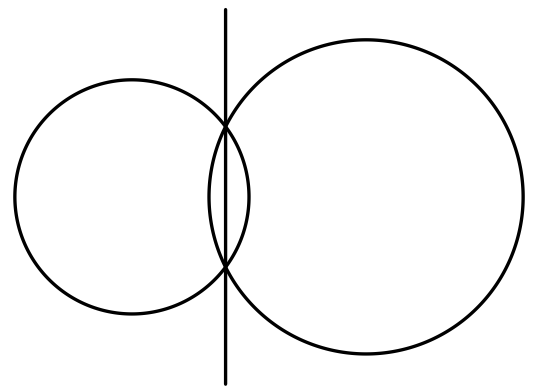
\includegraphics[scale=0.4]{p6.1}
		\caption{Un ejemplo de un eje radical}
	\end{figure}

\textbf{Ejercicio 9.} Use el Hecho 9 para deducir que un eje radical es siempre una l\'inea.
\\\\
Es bien sabido (y f\'acil de probar) que, dado tres c\'irculos distintos, sus ejes radicales de par en par o son concurrentes o son todos paralelos. Si los tres ejes radicales se encuentran en un punto en com\'un, decimos que ese punto com\'un de intersecci\'on es el $centro \ radical$ de los tres c\'irculos.

Por ejemplo, usando la Figura 6, vemos que $BC$ es el eje radical de los c\'irculos $ABCD$ y $BCQM$, $AD$ es el eje radical de los c\'irculos $ABCD$ y $ADQM$, y $QM$ es el eje radical de los c\'irculos $ADQM$ y $BCQM$. As\'i que las l\'ineas AD, BC, QM se encuentran en un punto en com\'un, $R$, el centro radical de los tres c\'irculos: $ABCD, ADQM, BCQM$.

\textbf{Hecho 10.} Usando la Figura 6. Los puntos $A,C,M,O$ son conc\'iclicos, y los puntos $B, D, M, O$ son conc\'iclicos.

\textbf{Ejercicio 10.} Probar el Hecho 10. (Esto es una persecusi\'on de \'angulos f\'acil)

\textbf{Hecho 11.} Usando la Figura 6. Las l\'ineas AC, BD, OM son concurrentes.
\\\\
$Prueba$. Considera los tres c\'irculos: $ABCD, AOCM, BODM$. Las l\'ineas $AC,BD,OM$ son los tres ejes radicales, y por lo tanto deben concurrir. \ $\square$
\newpage
\textbf{Ejercicio 11.} Muestre que $MO$ biseca a $\angle CMA$ y a $\angle BMD$
\begin{figure}[h]
	\centering
	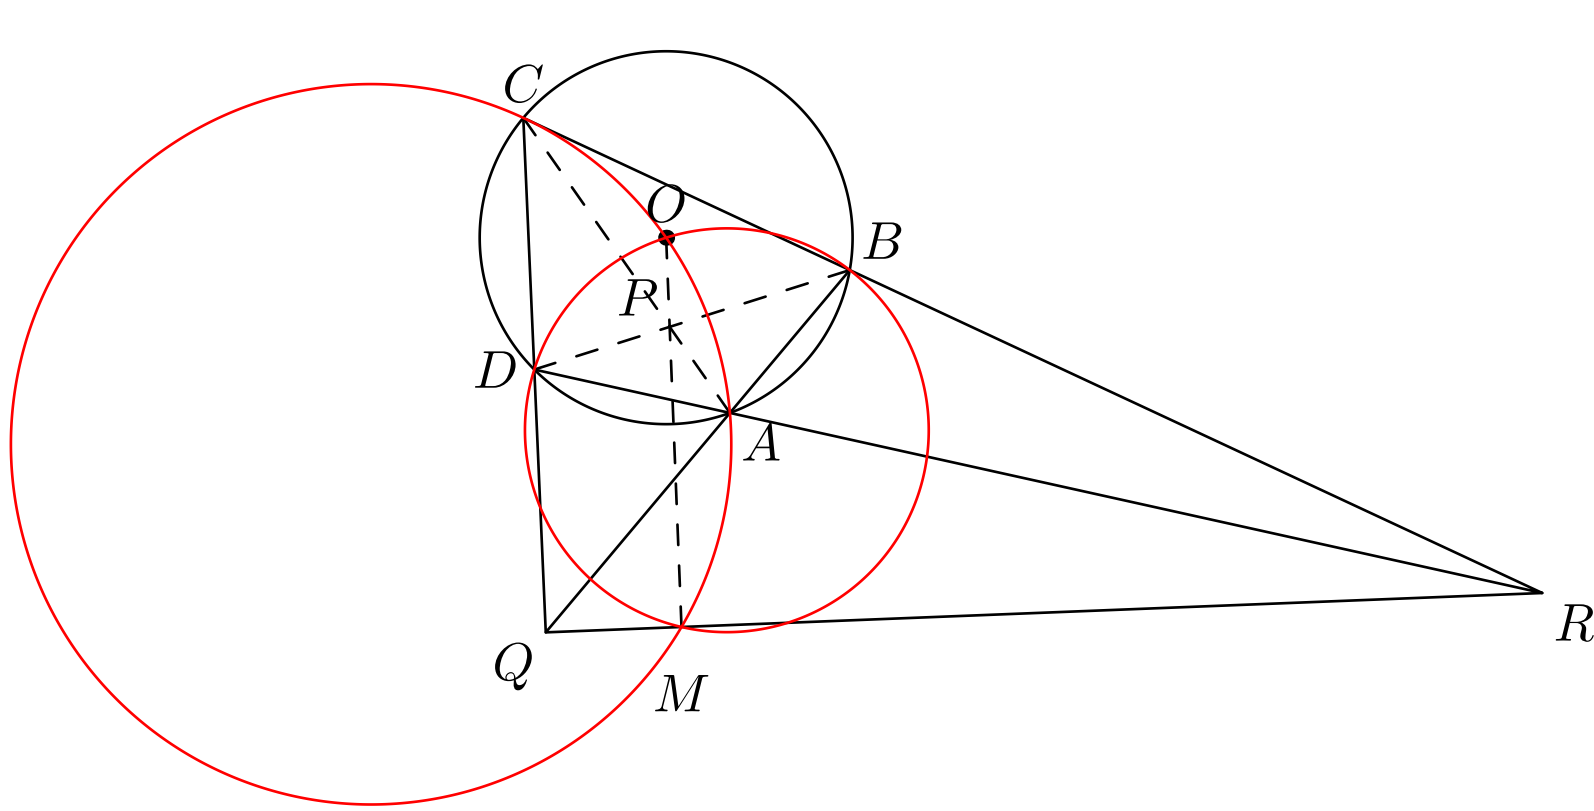
\includegraphics[scale=0.3]{p6.2}
	\caption{Diagrama para la prueba del Hecho 11.}
\end{figure}

\end{document}